\section{Анализ предметной области}

В данном разделе будет изложено видение \vk{} как системы мгновенного обмена
сообщениями; произведен краткий обзор существующих аналогов приложения; приведён
обзор инструментов \vk{} API для работы с личными сообщениями; сформулированы
требования к разрабатываемому программному средству.

\subsection{\vk{} как система мгновенного обмена сообщениями}

В настоящее время наблюдается тенденция переноса большого количества задач в
браузер. Это связано с активным развитием веб-технологий и появлением
возможностей реализовывать сложный и функциональный интерфейс, который будет
корректно функционировать в любом окружении с современным веб-браузером.

Применительно к предметной области это не даёт основания ожидать обратного
процесса (большого количества реализаций десктопного клиента такого веб-сервиса
как социальная сеть \vk{}). Полноценный клиент ограничен API социальной сети,
которое пока предоставляет доступ не ко всем функциям сайта, хотя большинство
функций в нем доступны. Более того на первый взгляд работа по повторной
реализации удобного интерфейса доступа к функциям сайта кажется бессмысленной (и
по сути является таковой), так как \vk{}, как впрочем и большинство социальных
сетей, изначально задумывались как продукт, доступный в любом окружении с
подключением к интернету и установленным веб-браузером и не требующий установки
дополнительного ПО.

Однако функциональность \vk{}, связанная с общением посредством личных
сообщений, требует дополнительного анализа, так как является далеко не первой
попыткой реализовать систему мгновенного обмена сообщениями и имеет в своей
основе механизм, который лишь недавно был перенесён в браузер.

Системы мгновенного сообщениями, часто представляющие собой самостоятельные
продукты, как правило имеют в своем составе центральный сервер, к которому
посредством клиентского ПО подключаются пользователи. Ранние сервисы такого типа
являлись мгновенными практически в прямом смысла слова, так как всё, что
печаталось пользователем, автоматически передавалось собеседнику, то есть был
виден весь процесс редактирования сообщения. Позже фаза создания и
редактирования сообщения была отделена от передачи, и у пользователя появилась
возможность отправлять уже отредактированные сообщения. Тем не менее
ориентированность на чат в реальном времени закрепила за данным классом программ
прилагательное <<мгновенный>>.

Программы данного класса всегда характеризовались обилием настроек, связанных с
уведомлениями о новых сообщениях, различными автоответчиками, группировкой
собеседников по различным критериям и интеграцией с операционной системой.
Доступ к функционалу мгновенного обмена сообщениями с помощью \vk{} через
браузер накладывает определенные ограничения на реализацию данного функционала.
Однако популярность \vk{} как браузерного мессенджера связана в первую очередь с
популярностью самой социальной сети, которая дает возможность собрать всю
переписку в одном месте.
Ещё совсем недавно хорошо известный мессенджер ICQ был в подобной ситуации, но
со временем был вытеснен более функциональными социальными сетями.

Популярность запросов <<мессенджер vk windows>>, <<vk windows>> и подобных им
доказывает, что совместить универсальность \vk{} с удобством классических
мессенджеров хотят многие пользователи. Немотря на это разнообразием клиентов
десктопный сегмент операционных систем похвастаться не может, чего нельзя
сказать об Android и iOS.

\subsection{Обзор аналогов}

Единственным официальным и полнофункциональным клиентом для \vk{}, работающим на
Windows, является приложение \textbf{ВКонтакте для Windows} (рисунок
\ref{fig:vk_windows}). Приложение поддерживает весь функционал сайта, доступный
через API, имеет поддержку вывода информационных уведомлений на рабочий стол и
возможность использования технологии live tiles, введенной в Windows 8. При этом
приложение имеет один серьёзный недостаток:
будучи выполненным для использования в Metro-режиме, оно поддерживается только
на операционных системах Windows 8.1 и новее. К тому же использование таких
приложений не является особенно удобным в операционных системах старше Windows
10. Несмотря на достаточно качественную реализацию функционала социальной сети,
нацеленность программы на использование её в Metro-режиме, а также наличие всё
тех же отвлекающих элементов, что и в веб-версии не позволяет использовать её в
качестве удобного клиента для мгновенного обмена сообщениями через \vk{}. При
этом стоит отметить хорошую адаптированность приложения под сенсорные дисплеи,
связанную с использованием Metro-дизайна.

\begin{figure}[ht] 
\centering
    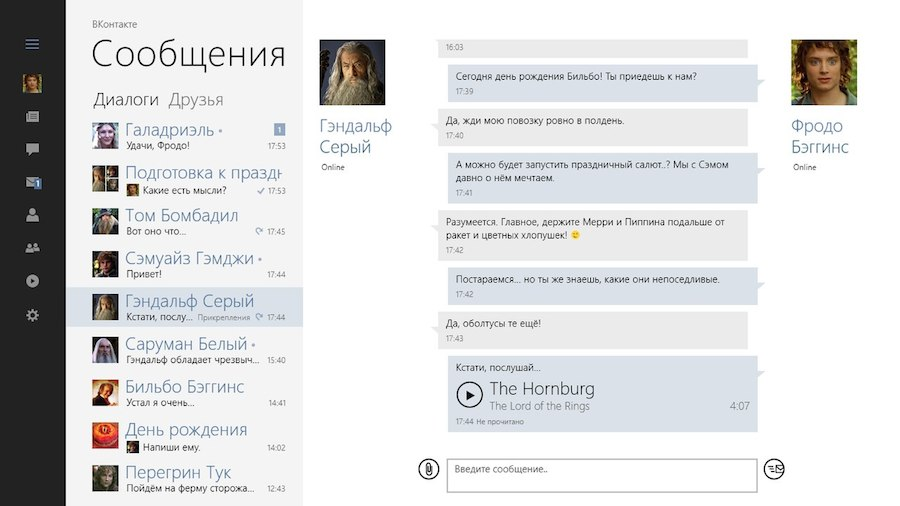
\includegraphics[scale=0.55]{vk_windows.jpg}
    \caption{ВКонтакте для Windows}
  	\label{fig:vk_windows}
\end{figure}

Неофициальных клиентов для \vk{} под Windows оказалось достаточно много, однако
лишь \textbf{Vk Quick Messenger} оказался в работоспособном состоянии и им
удалось успешно воспользоваться по назначению. Судя по информации со страницы
приложения и его функциональности, оно находится ещё на очень ранней стадии
разработки. При этом поледнее обновление официальной страницы было выполнено
достаточно давно, в связи с чем не приходится рассчитывать на активный процесс
разработки. Идея приложения и его интерфейс являются очень близкими к концепции
классического мессенджера (рисунок \ref{fig:vk_qm}). Имеется главное окно со
списком друзей из социальной сети, с которыми можно начать общение, и окно с
диалогами, разделенное на вкладки.
К сожалению, низкая функциональность делает приложение практически непригодным
для использования.
В приложении нет возможности загрузить и просмотреть историю уже имеющихся в
диалоге сообщений, а также отсутствует поддержка вложений. В ходе работы с
приложением также была зафиксирована низкая стабильность и частые аварийные
завершения.

\begin{figure}[ht] \centering 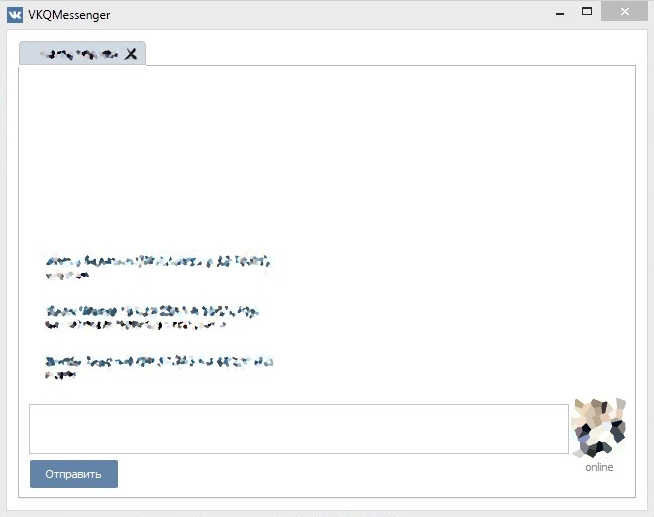
\includegraphics[scale = 0.5]{vk_qm.jpg}
	\caption{Окно диалога Vk Quick Messenger}
	\label{fig:vk_qm}
\end{figure}

Кроме специализированных приложений, работающих только с \vk{}, существует
многофункциональный мессенджер \textbf{QIP} (рисунок \ref{fig:qip}),
поддерживающий большое количество протоколов мгновенного обмена сообщениями и
многие популярные социальные сети.
К сожалению, поддержка функционала личных сообщений через \vk{} в нём
реализована не полностью.
Отсутствует, например, поддержка пересылки сообщений, не реализовано отображение
всех типов вложений, не продуман функционал пометки входящих сообщений
прочитанными, также собеседнику не отправляется уведомление о наборе текста.

\begin{figure}[hb!] \centering 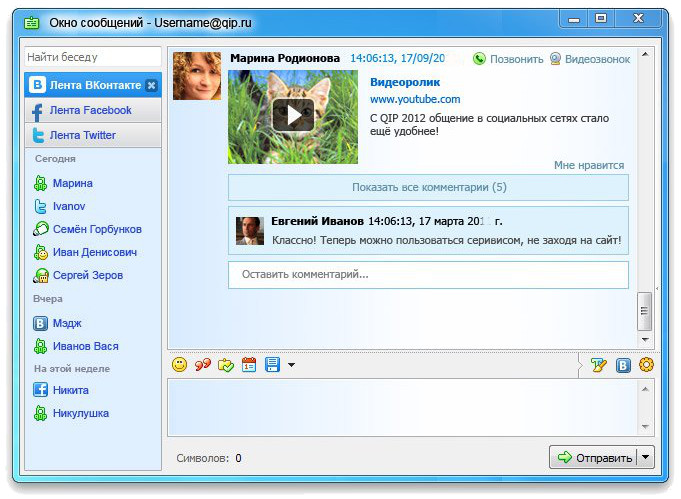
\includegraphics[scale = 0.5]{qip.png}
	\caption{Лента \vk{} в QIP}
	\label{fig:qip}
\end{figure}

Результат сравнения имеющихся аналогов с разрабатываемым приложением \vkapp{}
приведён в таблице \ref{table:functions_comparing}.

\begin{table}[h] \caption{Сравнение функциональности существующих аналогов с
разрабатываемым приложением \vkapp{}}
\label{table:functions_comparing}
\centering
     \begin{tabular}{ | >{\centering}m{0.35\textwidth} 
					  | >{\centering}m{0.2\textwidth} 
					  | >{\centering}m{0.11\textwidth} 
					  | >{\centering}m{0.05\textwidth}
					  | >{\centering\arraybackslash}m{0.155\textwidth}|}
	\hline Функция & \vk{} для Windows & VK QM & QIP & \textbf{\vkapp{}}\\
  	\hline Пересылка сообщений & + & - & - & +\\
  	\hline Отображение вложений & + & +/- & +/- & +\\
  	\hline Прикрепление вложений & + & +/- & +/- & +\\
  	\hline Пометка сообщений прочитанными & + & - & - & +\\
  	\hline Классический интерфейс мессенджера & - & + & + & +\\
  	\hline Уведомления \\ о новых сообщениях \\ на рабочем столе  & + & - & + &
  	+\\
  	\hline Информирование о наборе сообщения собеседником & + & - & + & +\\
  	\hline Отсутствие отвлекающего функционала \\ социальной сети & - & + & +/- &
  	+
  	\\
  	\hline Поддержка \\ групповых диалогов & + & - & + & + \\
  	\hline Синхронизация \\ истории сообщений \\ с учетной записью & + & - & - &
  	+
  	\\
  	\hline
  \end{tabular}
\end{table}

При составлении таблицы учитывался
весь запланированный функционал, реализация некоторых функций возможна в
версиях, которые будут разработаны вне данного курсового проекта.

\subsection{Обзор инструментов API \vk{} для работы с личными сообщениями}
\label{sec:vk_api_description}

API \vk{} обеспечивает удобный доступ ко всем функциям
социальной сети, связанной с личными сообщениями. 

Перед использованием большинства функций API необходимо произвести авторизацию
пользователя и получить ключ доступа для работы с социальной сетью. Возможны два
способа авторизации: OAuth-авторизация и прямая авторизация.
Первый способ требует перенаправления на веб-страницу \vk{}, содержащую форму
ввода учётных данных и запрос на разрешение доступа авторизирующемуся приложению
к определенным разделам учётной записи. Второй способ доступен приложению только
после предварительного одобрения администрацией и предполагает авторизацию
напрямую по логину и паролю пользователя.

По умолчанию API возвращает результаты своей работы в формате JSON, который
является удобным форматом сериализации структур данных любой сложности. JSON
легко отображается в словари и списки и имеет хорошую поддержку в различных
фреймворках.

Личное сообщение в API \vk{} представлено объектом message,
содержащим следующую информацию:
\begin{itemize}
  \item идентификатор сообщения в виде целого числа;
  \item идентификатор пользователя, в диалоге с которым находится сообщение;
  \item идентификатор автора сообщения;
  \item дата отправки сообщения;
  \item информация о прочитанности сообщения;
  \item текст сообщения;
  \item вложения, прикрепленные к сообщению (в том числе пересланные сообщения).
\end{itemize}

Сообщения из групповых диалогов имеют следующие дополнительные поля:
\begin{itemize}
  \item идентификатор группового диалога;
  \item информация о настройках уведомлений;
  \item название диалога;
  \item идентификатор создателя диалога;
  \item количество участников диалога;
  \item ссылки на изображение диалога в различном разрешении.
\end{itemize}

Также в групповом диалоге могут присутствовать служебные сообщения,
информирующие о добавлении или исключении пользователей, а также смене названия
или изображения диалога.

C помощью функций API с сообщениями можно выполнять следующие действия:
\begin{itemize}
  \item получить диалоги указанного пользователя;
  \item получить личные сообщения указанного пользователя;
  \item получить сообщения по их идентификаторам;
  \item произвести поиск по личным сообщениям;
  \item отправить сообщение;
  \item удалить сообщение;
  \item отметить сообщение как прочитанное;
  \item создать групповой диалог;
  \item изменить название и фотографию группового диалога.
\end{itemize}

Несмотря на широкую функциональность API, для чата в реальном времени
используется другой, более быстрый механизм LongPoll запросов. Принцип работы
LongPoll соединения заключается в том, что сервер, получив запрос, удерживает
его до тех пор, пока не произойдёт новое событие или не истечёт время, указанное
в качестве параметра запроса. Для идентификации момента, с которого необходимо
возвращать события, используется специальный числовой параметр,
передаваемый серверу при каждом новом запросе и возвращаемый в качестве ответа
на каждый такой запрос.

LongPoll сервер возвращает события следующих типов:
\begin{itemize}
  \item получение новых сообщений;
  \item изменение состояния прочитанности сообщений;
  \item изменение онлайн статуса пользователя из списка друзей;
  \item набор текста сообщения собеседником;
  \item изменение параметров беседы.
\end{itemize}

Как уже отмечалось выше, личные сообщения поддерживают прикрепление различных
вложений. Возможны следующие вложения: фотография, видеозапись, аудиозапись,
документ, запись на стене, комментарий, стикер. Все эти вложения представлены в
виде соответствующих объектов, наподобие объекта message для личных сообщений.

Из данного обзора видно, что \vk{} предоставляет разработчикам широкие
возможности по удобному взаимодействию с социальной сетью. Присутствуют все
необходимые инструменты для разработки программного средства для мгновенного
обмена сообщениями на базе данной социальной сети.

\subsection{Постановка задачи}

Целью данного курсового проекта является разработка кроссплатформенного
программного средства \vkapp{} для мгновенного обмена сообщениями через
социальную сеть \vk{}. В программе планируется реализовать следующие функции:
\begin{itemize}
  \item отправка и получение сообщений в режиме реального времени;
  \item пересылка сообщений;
  \item правильная пометка сообщений как прочитанных;
  \item поддержка уведомлений о наборе сообщения;
  \item поддержка основных типов вложений;
  \item синхронизация истории сообщений с учетной записью в социальной сети;
  \item отображения списка друзей пользователя для создания новых диалогов;
  \item настраиваемые уведомления о новых сообщениях;
  \item полная поддержка групповых диалогов.
\end{itemize}

Программное средство должно корректно вести себя в случае нарушения соединения с
интернетом или неполадок на стороне социальной сети. С целью обеспечения
кроссплатформенности разработка будет вестись на языке программирования C++ с
использованием фреймворка Qt.








